%*******************************************************************************
%****************************** Second Chapter *********************************
%*******************************************************************************

\chapter{Contesto tecnologico} \label{chap:tecnologico}

\ifpdf
    \graphicspath{{Chapter2/Figs/Raster/}{Chapter2/Figs/PDF/}{Chapter2/Figs/}}
\else
    \graphicspath{{Chapter2/Figs/Vector/}{Chapter2/Figs/}}
\fi


\section[Introduzione ai droni]{Introduzione ai droni}
I droni, detti anche Unmanned Aerial Vehicles (UAVs) o Unmanned Aircraft Systems (UAS), possono essere definiti, nella maniera più generale, come dei velivoli aerei privi di equipaggio umano a bordo. Essi vengono pilotati in remoto da personale specializzato a terra (Ground Control Station, \figurename\ \ref{fig:uavpilotavoidbadweather}), oppure dispongono di autonomia decisionale. 
%
\begin{figure}
	\begin{center}
		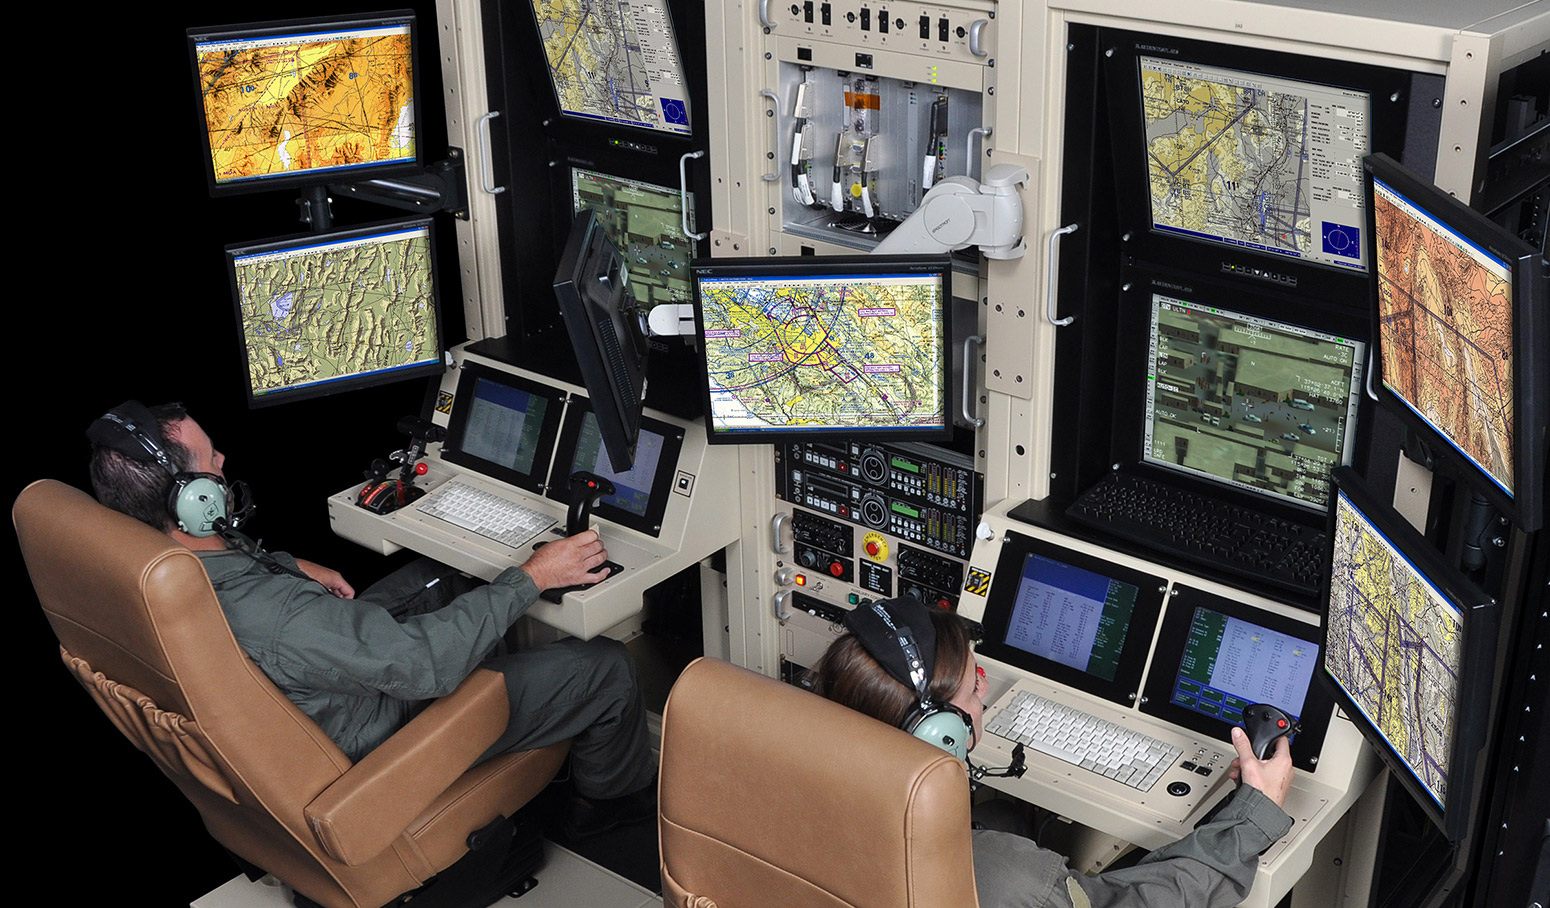
\includegraphics[scale=0.15]{uavpilotavoidbadweather}
	\end{center}
	\caption{Pilotaggio di un drone militare da remoto.\label{fig:uavpilotavoidbadweather}}
\end{figure}
%
Il volo autonomo è reso possibile tramite tecniche di intelligenza artificiale, utilizzando appositi sensori montati sul drone (come GPS o videocamere) per individuare ostacoli, conoscere la propria posizione e pianificare la rotta, spesso organizzata in waypoints. 
L'autonomia può essere completa, nel caso in cui tutte le decisioni sul movimento e le azioni sono elaborate dal computer di bordo, oppure parziale, in cui il computer di bordo interviene solo in particolari situazioni, ad esempio quando il drone perde la connessione con il pilota. \\

\subsection[Cenni storici]{Cenni storici}
Gli UAV sono nati in ambito puramente militare, per compiere missioni offensive o di ricognizione in cui non si poteva garantire l'incolumità del pilota; il loro sviluppo, portato avanti soprattutto dagli Stati Uniti, Israele e dal Regno Unito, ha proseguito di pari passo con la corsa agli armamenti durante le grandi guerre del 1900. \\
I primi tentativi di realizzare velivoli senza pilota risalgono al periodo della Prima Guerra Mondiale, con l'obiettivo di creare degli “aerei bomba” (\figurename\ \ref{fig:Kettering_Bug}), che in futuro si sarebbero evoluti negli attuali missili teleguidati. 
%
\begin{wrapfigure}{R}{0.5\textwidth}
	\begin{center}
		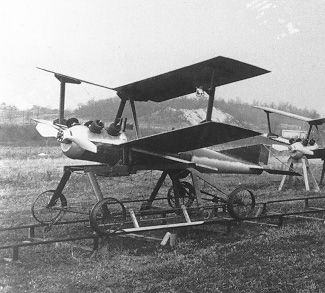
\includegraphics[scale=1.1]{KetteringBug}
	\end{center}
	\caption{Kettering Bug, uno dei primi prototipi di UAV militare, 1918.} \label{fig:Kettering_Bug}
\end{wrapfigure}
%
Furono perfezionati durante la Seconda Guerra Mondiale, e usati anche come bersagli mobili per addestrare gli addetti alla difesa contraerea, mentre conobbero un forte sviluppo durante i conflitti successivi agli anni '50, in cui vennero impiegati sia come armi offensive che come ricognitori per rimediare alle forti perdite di vite umane subite dall'aeronautica militare.  \\
I droni militari moderni sono nati a partire dagli anni '90: grazie al forte sviluppo dell'elettronica, la miniaturizzazione dei componenti e il conseguente abbattimento dei costi, l'interesse nei loro confronti è cresciuto sempre di più, fino a renderli una componente rilevante in molti eserciti contemporanei \cite{keane2013brief}.

\subsection[Ambiti d'uso]{Ambiti d'uso}
Come già accennato, in ambito militare i droni sono impiegati principalmente come ricognitori o bombardieri. 
Un nuovo metodo di impiego li vede coinvolti nel fornire supporto logistico alle truppe a terra, sia come trasporto attrezzatura sia come ponte radio per comunicazioni sicure tra squadre rimaste isolate. \\
L'impiego dei droni in campo civile invece è estremamente recente, e si studiano continuamente nuovi ambiti in cui poterli impiegare. 
Generalmente in questo campo si impiegano UAV di dimensioni ben più ridotte rispetto alle controparti militari, spesso veri e propri velivoli aerei. \\
Oltre allo scopo ricreativo e di fotografia aerea, sono stati impiegati con successo in agricoltura, per monitorare la salute del raccolto (la cosiddetta agricoltura di precisione) o irrigarlo, per ispezionare linee elettriche, condutture o edifici lesionati, nella sorveglianza domestica o di ampie aree geografiche, come supporto alle forze dell'ordine, nel monitoraggio della qualità ambientale dell'aria, come rilevatori di concentrazione di sostanze pericolose per l'uomo in seguito a disastri ambientali, nel supporto alle squadre di soccorso per individuare feriti o dispersi e per portare il prima possibile kit medici e defibrillatori agli operatori sanitari, come corrieri espressi per le spedizioni Amazon \cite{amazon}, contro il bracconaggio e per combattere incendi \cite{dronespeak}. 

\subsection[Tassonomia]{Tassonomia}
Non esiste un metodo unico per poter categorizzare efficacemente i droni, in quanto essi variano enormemente per caratteristiche tecniche e ambiti di utilizzo. Essi infatti possono essere suddivisi per:
\begin{itemize}
	\item Ambito:
		\begin{itemize}
			\item Militare: droni da combattimento, ricognitori, segnalatori di bersagli o esche anti-missile (decoys);
			\item Logistico: droni in grado di trasportare merci o attrezzature;
			\item Ricerca e sviluppo;
			\item Civile e commerciale: modellismo, riprese aeree, raccolta dati, supporto alle forze di soccorso, sorveglianza.
		\end{itemize}
	\item Altitudine e portata massimi \cite{uasglobal} :
		\begin{itemize}
			\item Portatili: fino a 600 m di altitudine e portata di 2 km; 
			\item Corto raggio: fino a 1500 m di altitudine e 10 km di portata;
			\item NATO e tattici: tra i 3000 e i 5000 m di altitudine e un range massimo di 160 km;
			\item Medio ed ampio raggio: fino a 9000 m e oltre i 200 km di portata. Oltre i 9000 m vengono definiti ad ampio raggio;
			\item Ipersonici:  fino a 15000 m, range superiore ai 200 km.
		\end{itemize}
	\item Dimensione e peso: qui la categorizzazione è meno precisa, in quanto ogni Paese definisce i propri standard:
		\begin{itemize}
			\item MAV (Micro Air Vehicle): droni che possono stare nel palmo di una mano. Recenti sviluppi hanno portato a modelli grandi pochi centimetri e del peso di alcuni grammi;
			\item SUAV (Small UAV): droni sufficientemente piccoli da essere trasportati da una persona e del peso non superiore ai 20-25 kg;
			\item HUAV (Heavy UAV):  in questa categoria rientrano tutti quei droni la cui struttura è comparabile, in dimensioni, a quella di un velivolo aereo. Hanno elevate capacità di trasporto e possono coprire elevate distanze prima di necessitare di rifornimento. Il loro uso è prevalentemente per scopi militari o di rilevamento.
		\end{itemize}
	\item Configurazione di volo: determina la struttura, la tipologia di motori e gli ambiti in cui può essere impiegato con maggior efficienza. Le principali versioni sono mostrate in \figurename\ \ref{fig:struttura}: 
		\begin{itemize}
			\item Multi-rotori: droni che impiegano più di due rotori per il volo. Hanno avuto ampia diffusione in ambito commerciale e modellistico grazie alla semplicità di costruzione, alla stabilità del volo e alla maggior capacità di carico. Le principali limitazioni sono bassa autonomia di volo e ridotta velocità;
			\item Ad ala fissa: sono equipaggiati con ali simili a quelle degli aerei, dispongono di buona autonomia ma non sono capaci di effettuare volo stazionario. Inoltre non sono generalmente in grado di decollare e atterrare in maniera autonoma, richiedendo sistemi simili a catapulte e paracadute;
			\item A rotore singolo: dispongono di un solo rotore, rendendoli concettualmente simili a un elicottero. Ciò li rende energeticamente molto più efficienti rispetto ai multi-rotore, a discapito di una maggiore complessità di costruzione e minore stabilità di volo;
			\item Ibridi: i più recenti, combinano la struttura ad ala fissa con uno o più rotori, posizionati in coda o verso il suolo, ottenendo i benefici di entrambe le configurazioni. 
		\end{itemize}
\end{itemize}
%
\begin{figure}
	\centering
	\begin{subfigure}[b]{0.4\textwidth}
		\centering
		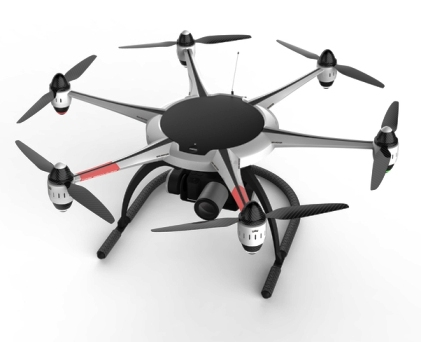
\includegraphics[scale= 1]{sixrotor}
		\caption{Multi-rotore}
		\label{fig:multirotor}
	\end{subfigure}
	%
	\begin{subfigure}[b]{0.4\textwidth}
		\centering
		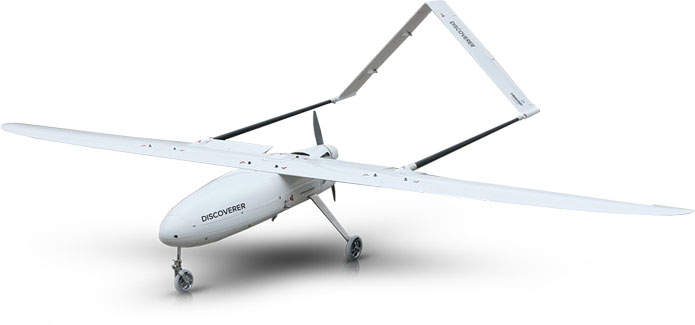
\includegraphics[scale= 0.2]{fixed}
		\caption{Ad ala fissa}
		\label{fig:fixed}
	\end{subfigure}
	%
	\begin{subfigure}[b]{0.4\textwidth}
		\centering
		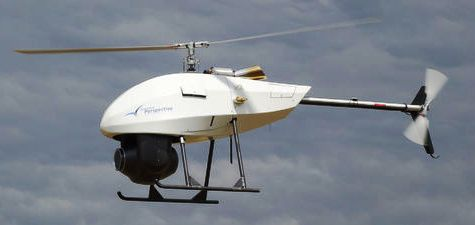
\includegraphics[scale= 1.5]{singlerotor}
		\caption{Singolo rotore}
		\label{fig:singlerotor}
	\end{subfigure}
	%
	\begin{subfigure}[b]{0.4\textwidth}
		\centering
		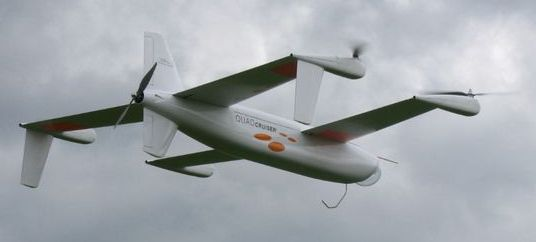
\includegraphics[scale = 0.39]{hybrid}
		\caption{Ibrido}
		\label{fig:hybrid}
	\end{subfigure}
	\caption{Principali configurazioni di volo dei droni}
	\label{fig:struttura}
\end{figure}
%
\subsection[Struttura]{Struttura}
La struttura di un drone, evidenziata in \figurename\ \ref{fig:uavstructure} è generalmente ricorrente, e può essere schematizzata nelle seguenti componenti \cite{Sahingoz2014}:

\begin{itemize}
	\item Fusoliera: l'assenza di equipaggio a bordo permette di poterla costruire con materiali più leggeri ed economici. Dimensione e forma variano grandemente in base alla funzionalità del drone e al peso che deve trasportare;
	\item Alimentazione: i droni di ridotta dimensione, come i MAV e gli SUAV, sono generalmente alimentati da batterie, mentre quelli più grandi richiedono i motori convenzionali di un aereo;
	\item Sensori: i sensori che il drone monta ne definiscono le funzionalità e le capacità di volo autonomo. Possono essere usati per raccogliere dati (sensori ambientali, fotocamere, videocamere), per la guida del drone da remoto, per evitare collisioni con ostacoli, per la navigazione autonoma (GPS, giroscopi, altimetri, accelerometri);
	\item Attuatori: sono i dispositivi, generalmente elettronici, che comandano i motori del drone e ne regolano l'assetto;
	\item Payload: è l'equipaggiamento trasportato dal drone, ed include sensori, trasmittenti, attrezzature, armi, etc. Generalmente il payload è contenuto in uno spazio interno apposito, per non influire sulle capacità aerodinamiche del mezzo;
	\item Computer di bordo e software: i droni sono dispositivi real-time, e sono equipaggiati con una o più unità di calcolo (microcontrollori, single-board computers, sistemi embedded, etc.)  per gestire il volo autonomo e i processi di decision-making. Le capacità di elaborazione degli UAV quindi crescono di pari passo con lo sviluppo e la miniaturizzazione dell'hardware;
	\item Sistemi di comunicazione: i sistemi di comunicazione del drone sono generalmente ad onde radio, e possono avvenire con l'operatore a terra in maniera diretta o indiretta (tramite un satellite o un altro velivolo), in base alla reciproca distanza. Il flusso di comunicazione è tipicamente composto in uplink dai comandi dell'operatore, e in downlink da segnali video, telemetria o rilevazioni dei sensori. Molti  MAV e SUAV comunicano via Wi-Fi, rendendo possibile pilotarli tramite smartphone o tablet.  
\end{itemize}
%
\begin{figure}
	\begin{center}
		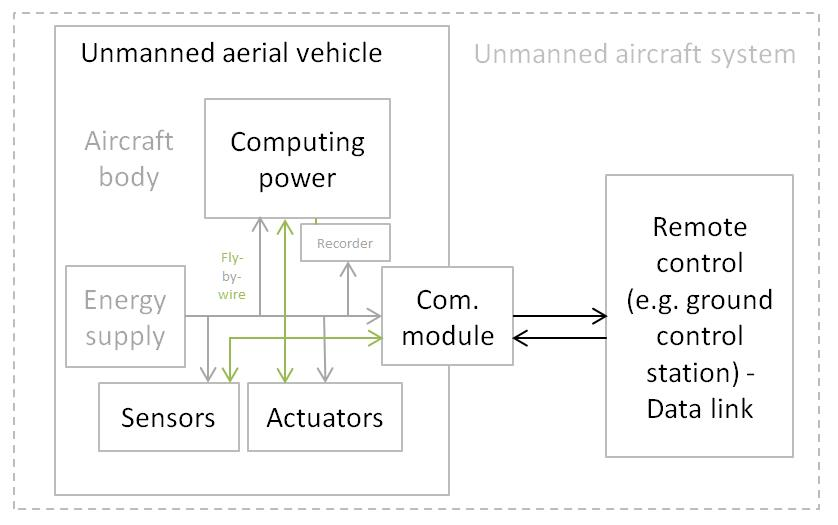
\includegraphics[scale=0.5]{uavstructure}
	\end{center}
	\caption{Schema a blocchi dei principali componenti di un drone} \label{fig:uavstructure}
\end{figure}
%
\subsection[Autonomia di volo]{Autonomia di volo} \label{sect:autonomia}
Una delle attuali sfide nel mondo degli Small UAV è l'incremento del loro tempo di volo, che generalmente non supera i 10-20 minuti prima di dover effettuare la ricarica della batteria. \\
Forza del vento, tipologia dei sensori installati, peso del drone e frequenza di movimento sono i principali fattori che incidono sul consumo della batteria. 
È possibile caricare il drone con più batterie in parallelo, ma più batterie equivalgono a maggior peso da sollevare e a un conseguente maggior consumo di energia da parte dei motori, rendendo quindi risibile il contributo di più batterie alla durata di volo.\\
Negli ultimi anni è stata esplorata la strada dei pannelli solari come fonte energetica ausiliaria per incrementare l'autonomia di volo (\figurename\ \ref{fig:solar}). 
%
\begin{figure}
	\centering
	\begin{subfigure}[b]{0.4\textwidth}
		\centering
		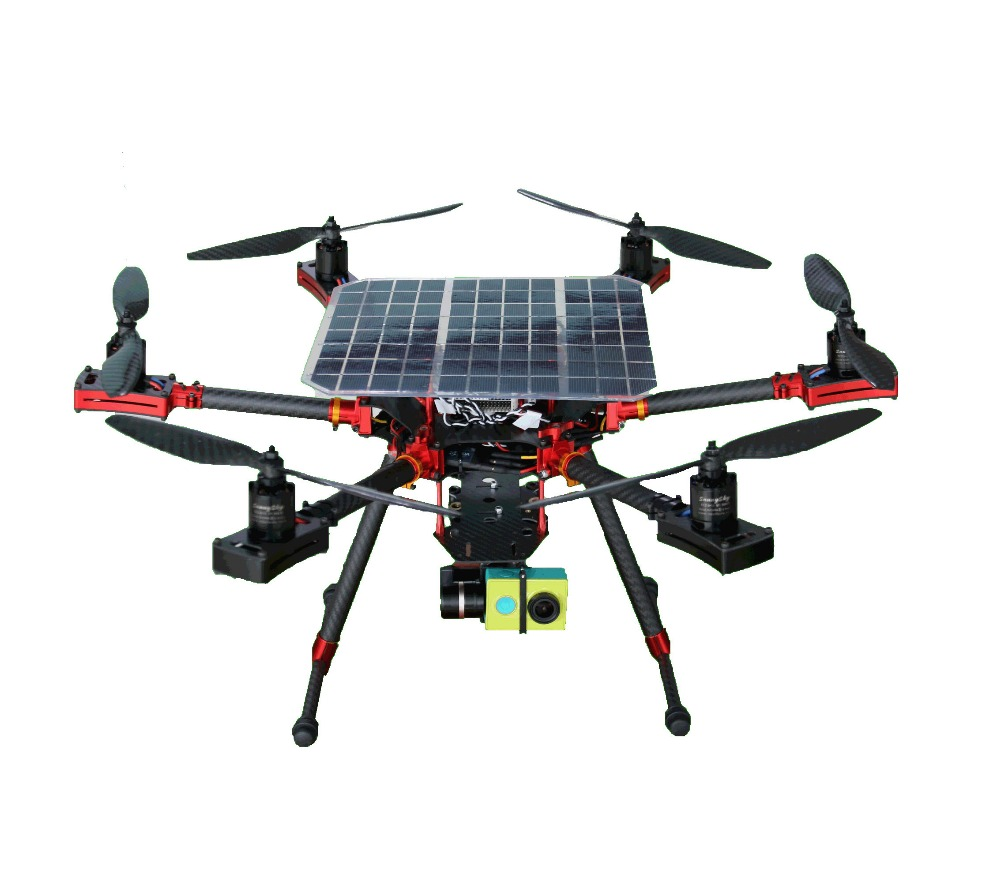
\includegraphics[scale= 0.15]{solarquad}
		\caption{Multi-rotore solare}
		\label{fig:solarquad}
	\end{subfigure}
	%
	\begin{subfigure}[b]{0.4\textwidth}
		\centering
		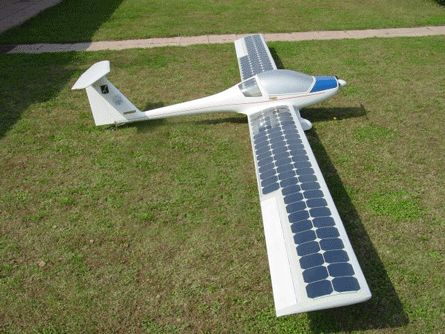
\includegraphics[scale= 0.4]{solarfixed}
		\caption{Ad ala fissa solare}
		\label{fig:solarfixed}
	\end{subfigure}
	\caption{Prototipi di droni ad energia solare}
	\label{fig:solar}
\end{figure}
%
I risultati migliori, seppur ancora lontani dall'autonomia energetica, sono stati ottenuti sui droni ad ala fissa \cite{newatlas} ricoprendo le ali di pannelli, mentre sui quadrirotori l'ingombro dell'attrezzatura aggiuntiva causava un effetto vela che riduceva la stabilità in volo \cite{diydrones}.\\ Se in campo commerciale ed amatoriale i risultati sono stati poco incoraggianti, non è andata così nel campo dei grandi velivoli: seppur guidato da un pilota, il progetto Solar Impulse 2, un aereo completamente alimentato dall'energia solare, ha completato il giro del mondo nell'estate del 2016 \cite{theguardian}, mentre Facebook sta attivamente testando l'uso di droni solari per fornire connettività a internet ai Paesi del Terzo Mondo con il progetto Aquila \cite{fbaquila}.\\

\section[Reti ad-hoc]{Reti ad-hoc}
Una rete Ad-hoc è una tipologia di WLAN decentralizzata in cui è assente la tradizionale infrastruttura delle reti managed (AP, router, switch, etc.), in quanto sono gli stessi nodi a occuparsene, agendo come routers. \\
La rete ad-hoc consiste in un gruppo di client mobili che formano spontaneamente una rete temporanea, dinamica e auto-configurante (ad esempio, per comunicare o condividere dati). 
Ciascun nodo potrà comunicare direttamente con tutti quelli entro il suo range trasmissivo, e tramite multi-hop con quelli al di fuori di esso (\figurename\ \ref{fig:manet}). \\
%
\begin{figure}
	\begin{center}
		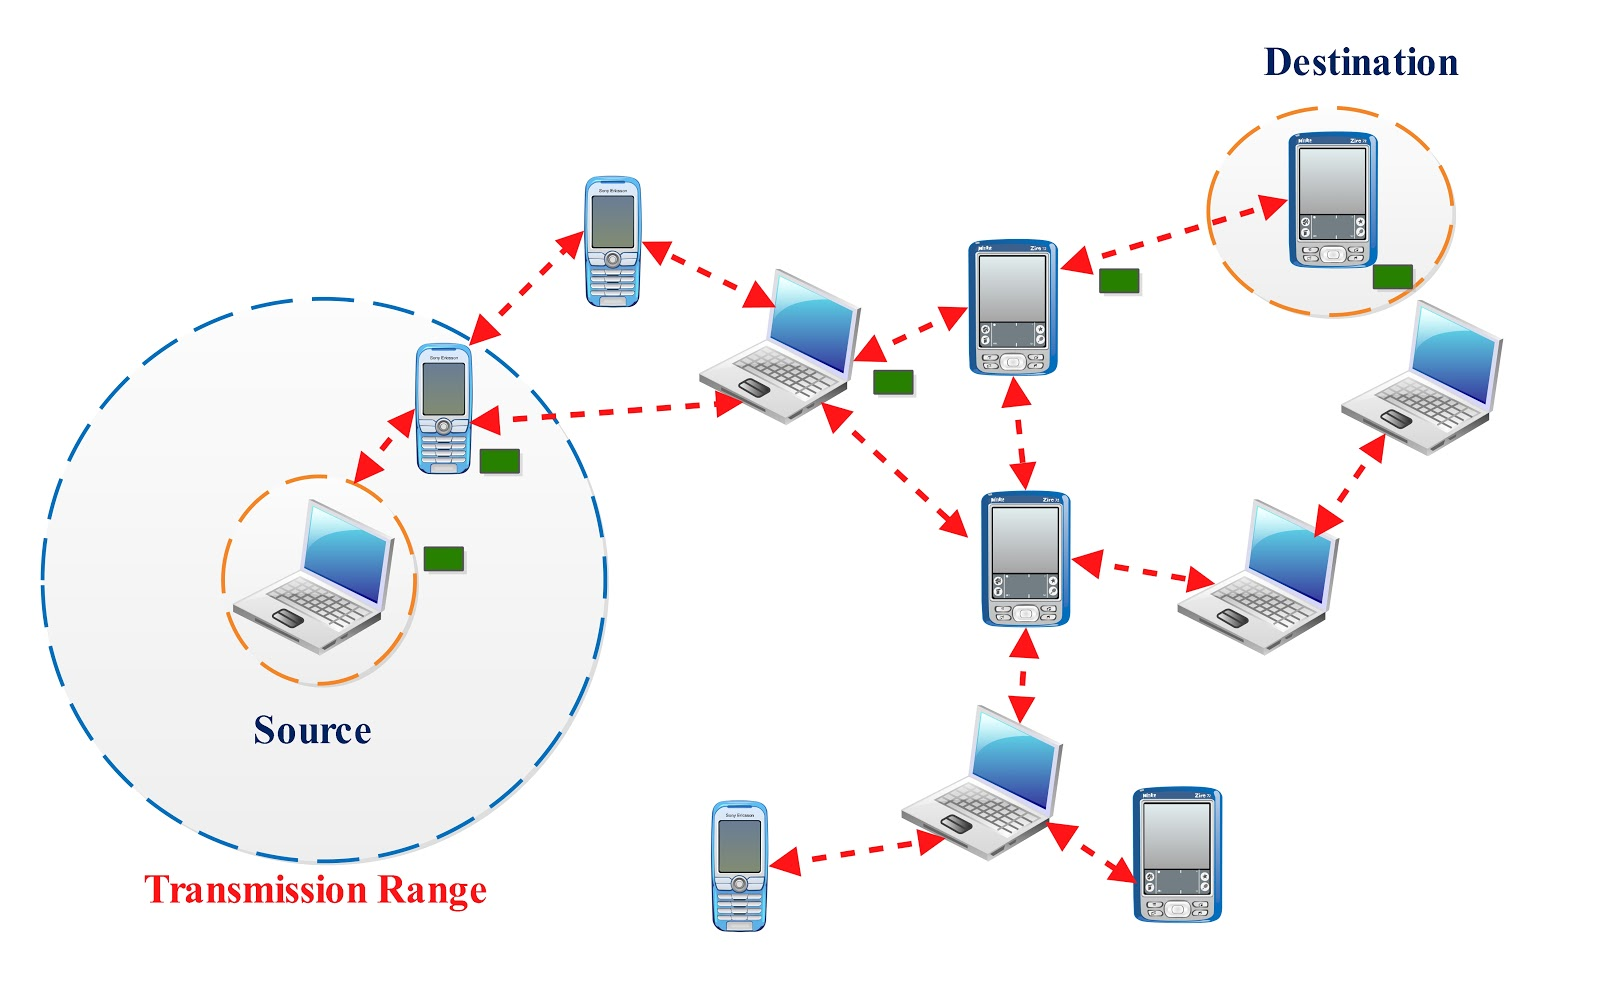
\includegraphics[scale=0.2]{manet}
	\end{center}
	\caption{Esempio di comunicazione multi-hop in rete ad-hoc.} \label{fig:manet}
\end{figure}
%
Poiché i client sono liberi di muoversi, la topologia di queste reti tende a cambiare velocemente e in maniera non prevedibile: possono verificarsi variazioni di routes, partizionamento del grafo di rete, fluttuazioni nella capacità dei link, con conseguente perdita di pacchetti, perciò i protocolli di rete devono avere un alto grado di adattabilità e reattività, per  monitorare lo stato dei link e regolare i flussi di traffico di conseguenza.
L'assenza di infrastruttura di routing dedicata richiede che il network management sia distribuito tra tutti i nodi, per esempio tramite flussi di traffico di controllo, aggiungendo un ulteriore livello di complessità. \\
Le reti ad-hoc sono tipicamente impiegate in quelle situazioni in cui l'infrastruttura di rete è assente, inadatta o compromessa: alcuni casi d'uso possono essere la condivisione di dati in un meeting, comunicazioni militari, networking, servizi veicolari (trasmissione di news, intensità del traffico, musica, etc.), gaming, o l'instaurazione di sistemi di comunicazione per le squadre di soccorso in seguito a calamità naturali \cite{7402025}. \\
I principali vantaggi delle reti ad-hoc sono la capacità di auto-configurazione dei nodi, richiedendo un intervento minimo dell'utente, la velocità di deployment, il self-healing, ovvero la capacità della rete di riconfigurarsi autonomamente in seguito a un cambio della sua topologia, la scalabilità e i costi ridotti dovuti dall'assenza dell'infrastruttura.\\
I principali svantaggi di questo tipo di architettura sono la necessità di un elevato grado di adattabilità dei protocolli, a causa dei frequenti cambi di topologia nella rete, l'eterogeneità dei client, in quanto le diverse capacità di trasmissione, ricezione e calcolo dei dispositivi possono causare link asimmetrici, la dipendenza dei client dalla batteria del loro device, la cui durata viene ulteriormente ridotta dalle funzionalità di routing, e la vulnerabilità ad attacchi, a causa dell'assenza di una struttura centrale di autenticazione. \cite{jayakumar2007ad}
\\
In particolare, anche il power management dei nodi può influenzare la topologia della rete: un client può scegliere se aumentare la potenza di trasmissione (e il suo range, di conseguenza) per spedire direttamente un pacchetto al destinatario, oppure ridurla e fare affidamento sulla consegna multi-hop.\\
Questa scelta porta alla creazione e cancellazione di path, e alla modifica della topologia. 
Entrambi gli approcci hanno degli svantaggi: trasmettere a maggior potenza riduce il ritardo nella consegna dei messaggi, ma aumenta il consumo della batteria e riduce il throughput della rete, in quanto all'aumento del range corrisponde un aumento nella zona di interferenza, e tutti i nodi interni a questa area dovranno restare silenti fino al termine della trasmissione; la trasmissione a bassa potenza invece riduce il consumo della batteria e aumenta la capacità della rete, ma incrementa il ritardo medio dei pacchetti perché devono passare per più hop prima di giungere a destinazione. \\
Generalmente un compromesso viene raggiunto regolando dinamicamente la potenza trasmissiva e creando una condivisione di informazioni tra i protocolli di rete e i layer sottostanti. \cite{879383}

\subsection[Protocolli di routing]{Protocolli di routing}
I protocolli di routing vengono impiegati per determinare i path più efficienti (in termini di costi, ritardo, consumo energetico, etc.) attraverso i nodi della rete, che permettano ai messaggi di raggiungere la propria destinazione. \\
Il routing nelle reti ad-hoc deve tenere conto della mobilità dei nodi e delle loro limitate capacità energetiche e di calcolo. 
Questi due aspetti hanno soluzioni conflittuali, in quanto il primo richiede frequenti scambi di informazioni e aggiornamenti delle tabelle di routing, mentre il secondo li dovrebbe minimizzare, riducendo le trasmissioni e mantenendo tabelle di piccole dimensioni. \\
Si possono identificare due principali famiglie di protocolli di routing per le reti ad-hoc: protocolli proattivi e on demand.\\
I protocolli proattivi, di cui fanno parte le famiglie Link State e Distance Vector, effettuano un monitoraggio costante della rete e ne mantengono uno “stato” tramite le tabelle di routing. 
Al verificarsi di un cambiamento nella topologia, inviano messaggi (control traffic) agli altri nodi con le correzioni da apportare alle tabelle.\\ Permettono un rapido inoltro dei pacchetti grazie alle informazioni sempre aggiornate, ma la presenza costante di traffico di controllo introduce un overhead che cresce con la frequenza dei cambi di topologia, e in reti molto dinamiche può portare all'impossibilità di tenere traccia di tutti gli aggiornamenti delle stesse. Esempi di protocolli proattivi sono DSDV (Highly Dynamic Destination-Sequenced Distance Vector routing protocol), HSLS (Hazy Sighted Link State routing protocol), OLSR (Optimized Link State Routing Protocol) e STAR (Source Tree Adaptive routing protocol).\\
I protocolli on demand (o reattivi), invece, usano un approccio “lazy”, cioè non si preoccupano di mantenere una tabella di path aggiornati, ma richiedono il path di destinazione tramite flooding solo all'ultimo momento, quando sono presenti pacchetti che necessitano di essere instradati.
Questa tecnica permette una maggior scalabilità e non necessita di traffico di controllo, ma introduce un costante ritardo, detto setup delay, sul primo pacchetto che deve essere spedito a una nuova destinazione (che può diventare gravoso nel caso di traffico intermittente), e rende la rete vulnerabile ad attacchi basati sul flooding. Protocolli reattivi sono AODV (Ad hoc On Demand Distance Vector routing protocol) e DSR (Dynamic Source Routing) \cite{879383}. \\
Vi è poi una terza categoria, i protocolli ibridi, che cercano di combinare i vantaggi delle due famiglie, facendo routing proattivo per un ristretto gruppo di nodi (i nodi inizialid ella rete, o quelli considerati più “vicini”) e routing on demand su tutti gli altri. Un esempio è il protocollo ZRP (Zone Routing Protocol).\\

\subsection[Reti Infrastructure VS reti Ad-hoc]{Reti Ad-hoc VS Infrastructure}
Lo standard IEEE 802.11 per le Wireless Local Area Network (WLAN) prevede due principali modalità di funzionamento delle reti Wi-Fi: modalità infrastruttura (o managed) e modalità ad-hoc (\figurename\ \ref{fig:adhoc}). \\
%
\begin{figure}
	\begin{center}
		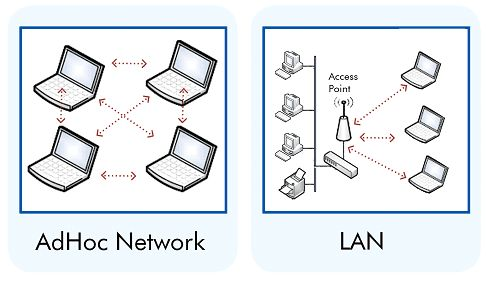
\includegraphics[scale=0.7]{adhoc}
	\end{center}
	\caption{Rete Infrastructure (a sinistra) e rete Ad-hoc (a destra).} \label{fig:adhoc}
\end{figure}
%
La modalità infrastruttura, generalmente più diffusa, prevede la presenza di base stations (Wireless Access Points, o APs) cui i client devono connettersi per poter comunicare tra loro. La comunicazione diretta client-client quindi non è ammessa, ma deve essere veicolata passando per l'AP. \\
Le base station, che svolgono una funzionalità di hub, a loro volta sono connesse, generalmente via cavo, all'infrastruttura centrale della rete e a un router. Esse sono generalmente fisse e forniscono connettività ai nodi client entro il proprio range.\\
Le reti infrastructure, come dice il nome, si appoggiano a una infrastruttura di rete, perciò sono generalmente pensate con un concetto di permanenza della stessa. 
La loro installazione e progettazione richiede costi in termini di denaro e tempo, mentre le reti ad-hoc non richiedono dispositivi aggiuntivi e si auto-configurano automaticamente in tempi rapidi. 
Le antenne degli AP sono generalmente più potenti di quelle equipaggiate da laptop o smartphone, permettendo quindi di comunicare a range superiori.  
Le reti ad-hoc in generale impongono ai client un maggior consumo di risorse di sistema per far fronte alla mobilità dei nodi e al conseguente cambio della topologia, mentre nelle reti managed gli APs sono generalmente fissi. Questo fattore risulta critico se si considera che i tipici client delle reti ad-hoc sono dotati di batteria, e di conseguenza in questa tipologia di rete la loro autonomia sarà minore.
Infine, le reti ad-hoc tendono a non scalare bene con il numero di client, a causa della maggior interferenza causata dalle numerose connessioni dirette tra client.

\section[Reti FANET]{Reti FANET}
Generalmente le reti ad-hoc vengono categorizzate in base alla tipologia dei client che le compongono. Le principali, schematizzate in \tablename\ \ref{tab:adhoc}  sono: MANETs (Mobile), VANETs (Vehicular), SPANs (Smartphone) e FANET (Flying). \\
Le reti FANET sono reti ad-hoc, ancora in fase sperimentale, tra droni equipaggiati con antenne radio, e possono essere viste come un sottoinsieme delle VANET (\figurename\ \ref{fig:fanet}), pur differendone sostanzialmente in termini di capacità, requisiti e problematiche. 
%
\begin{figure}
	\begin{center}
		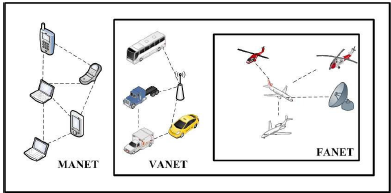
\includegraphics[scale=0.8]{fanet}
	\end{center}
	\caption{Tipologie di reti ad-hoc} \label{fig:fanet}
\end{figure}
%
Tali reti possono essere impiegate sia per lo scambio di informazioni tra droni, per esempio per coordinarsi nel volo autonomo in “stormo”, sia come relay per mettere in comunicazione client a terra. \\
Attualmente le FANET impiegano soprattutto gli heavy UAVs, per sfruttarne la maggior potenza di calcolo e trasmissione, oltre che la maggior autonomia di volo, ma grazie alla progressiva riduzione dei costi di produzione si sta sperimentando l'uso di molteplici Small UAVs. \\
Anche se il singolo SUAV ha capacità limitate, l'impiego di una squadra di droni  porta i seguenti vantaggi:
\begin{itemize}
	\item Aumenta la ridondanza, in quanto se un drone diventa offline i restanti possono riorganizzarsi e mantenere funzionante la rete, anche se a performance ridotte;
	\item Più droni possono parallelizzare il lavoro e ridurre i tempi della missione;
	\item Riduzione dei costi, impiegando più SUAVs economici rispetto un singolo e costoso HUAV;
	\item Aumenta la scalabilità, in quanto per coprire un'area di operazione maggiore basta aggiungere droni;
	\item Possono cooperare e sfruttare le reciproche funzionalità, utile soprattutto se equipaggiati in maniera differente gli uni dagli altri.
\end{itemize}
In una FANET si possono distinguere due modelli di comunicazione, che necessitano di protocolli differenti:
\begin{itemize}
	\item Comunicazione drone-drone: la comunicazione può essere diretta o multihop, e generalmente riguarda il coordinamento di volo e la cooperazione nel compiere un dato task;
	\item Comunicazione drone-infrastruttura: la comunicazione avviene tra il drone e una ground station (o un satellite) e generalmente consiste nel fornire i dati rilevati dai sensori del drone.
\end{itemize}
Come già accennato, le reti FANET rappresentano ancora un nuovo campo per la ricerca, e prima che possano raggiungere il loro potenziale devono essere risolte ancora molte problematiche. \\
In base alla tipologia di drone impiegato ci si può aspettare differenti gradi di mobilità dei nodi, dal volo stazionario del piccolo quadri-rotore all'alta velocità degli HUAVs, e quindi una diversa frequenza di variazione della topologia. 
Gli stessi droni possono viaggiare a velocità diversa, guastarsi o allontanarsi per ricaricarsi, creando partizionamenti e continue riorganizzazioni della rete. \\
Il consumo energetico è un altro fattore chiave nelle FANET: mentre nelle MANET i devices hanno  autonomie di svariate ore e nelle VANET i veicoli ricaricano la batteria grazie al movimento del mezzo, nelle FANET i piccoli droni possono restare in volo solo poche decine di minuti, perciò i protocolli di queste ultime devono minimizzare il consumo energetico, favorendo per esempio trasmissioni a bassa potenza e routing multihop. 
La presenza di molteplici droni aggiunge un ulteriore complessità, in quanto occorrono protocolli di coordinazione, organizzazione e path-planning.
Quest'ultimo consente ai droni di modificare il proprio percorso in reazione a cambiamenti dinamici, come la presenza di ostacoli. \\
Queste problematiche dimostrano che affinché le FANET possano essere impiegate efficacemente sono necessari nuovi  protocolli di comunicazione, coordinamento e cooperazione tra droni. \\
Nonostante le somiglianze tra le tipologie di rete, i protocolli usati nelle reti MANET e VANET generalmente non sono utilizzabili nelle FANET o hanno scarse performance, perciò occorre definire nuovi algoritmi di routing dedicati e prevedere modifiche ai layers MAC e network \cite{7317490}.

\begin{table}[]
	\small
	\centering
	\begin{tabular}{|p{2.2cm}|p{3cm}|p{3cm}|p{3cm}|}
		\hline
		& MANET                                                                                                         & VANET                                                                                                                                                                                                 & FANET                                                                                                                                     \\ \hline
		Tipo di nodo       & Mobile devices (tablet, laptop, smartphone, etc.)                                                             & Veicoli                                                                                                                                                                                               & Droni                                                                                                                                     \\ \hline
		Descrizione        & Dispositivi mobile in range tra loro si interconnettono in una rete ad-hoc, senza necessità di infrastrutture & Veicoli connessi tra di loro. La comunicazione avviene tra veicoli e tra veicoli e nodi di supporto (Roadside Units) disposti lungo la strada              & I droni costruiscono una rete ad-hoc fra di loro e i nodi a terra                                                                         \\ \hline
		Mobilità           & Lenta, generalmente al di sotto dei 2 m/s. Il pattern di movimento è tipicamente casuale                      & Alta velocità, in base alla tipologia di strada (urbana o aoutostradale). Il pattern di movimento è generalmente prevedibile in quanto vincolato dalla struttura della strada e dalle norme stradali. & Molto variabile, da stazionario a oltre i 100 m/s, a seconda della tipologia di drone. Il movimento può avvenire in due o tre dimensioni. \\ \hline
		Topologia          & Casuale, ad-hoc                                                                                               & A stella tra veicoli e infrastruttura stradale, ad-hoc tra i veicoli                                                                                                                                  & A stella tra droni e ground control, ad-hoc o a mesh tra droni                                                                            \\ \hline
		Dinamicità         & I nodi entrano ed escono dalla rete in maniera imprevedibile, frequenti partizionamenti                       & Maggior dinamicità rispetto la MANET, a causa della maggior velocità dei nodi e delle interferenze del traffico                                                                                       & Variabile, in base alla velocità relativa dei droni                                                                                       \\ \hline
		Vincoli energetici & Nodi con batteria, autonomia di alcune ore                                                                    & Batteria dei veicoli si ricarica con il movimento                                                                                                                                                     & Durata della batteria proporzionale alla dimensione dello UAV                                                                             \\ \hline
		Ambiti d'uso       & Distribuzione dell'informazione, hot spot internet, networking                                                & Informazioni di traffico, servizi location based, avvisi di emergenza                                                                                                                                 & Sorveglianza, salvataggio, distribuzione, monitoraggio                                                                                    \\ \hline
	\end{tabular}
	\caption{Confronto tra le diverse tipologie di reti ad-hoc} \label{tab:adhoc}
\end{table}

\subsection[Routing nelle FANET]{Routing nelle FANET}
Attualmente l'implementazione di algoritmi di routing per FANET ha seguito due strade: creazione di protocolli ad-hoc e modifiche di algoritmi preesistenti per MANET e VANET. \\
Si possono distinguere quattro tipologie di protocolli:
\begin{itemize}
	\item Statici: le tabelle di routing vengono pre-calcolate e caricate sul drone, per poi non essere più modificate fino al termine della missione. Questa forte limitazione può essere tollerata solo nei casi in cui la topologia della rete rimane fissa nel tempo. Esempi di questa famiglia di protocolli sono LCAD ( Load Carry and Deliver Routing) e il Multi-Level Hierarchical Routing;
	\item Proattivi: sono gli algoritmi table-driven per le reti ad-hoc precedentemente descritti. Impiegati nelle FANET garantiscono velocità nel routing, ma la loro necessità di scambiare traffico di controllo aggrava la già ridotta disponibilità di bandwith. Inoltre non sono adatti per reti di grandi dimensioni e in cui i nodi si muovono molto velocemente, poiché hanno tempi di reazione ai cambiamenti di topologia molto lunghi.
	\item Reattivi: precedentemente descritti come algoritmi on-demand, garantiscono un uso efficiente della banda in quanto non necessitano di traffico di controllo e scambi periodici di messaggi, ma introducono forti delay a causa della tipologia di traffico tipicamente intermittente delle FANET. 
	\item Ibridi: cercano di unire i vantaggi dei protocolli proattivi e reattivi, riducendo la latenza iniziale e l'overhead dei messaggi di controllo, e sono efficaci anche in reti di grandi dimensioni. 
\end{itemize}





% Uncomment this line, when you have siunitx package loaded.
%The SI Units for dynamic viscosity is \si{\newton\second\per\metre\squared}.

